
%(BEGIN_QUESTION)
% Copyright 2014, Tony R. Kuphaldt, released under the Creative Commons Attribution License (v 1.0)
% This means you may do almost anything with this work of mine, so long as you give me proper credit

A pair of split-ranged control valves work together to regulate natural gas pressure inside of a ``receiver'' vessel.  One valve admits natural gas into the receiver vessel to raise its pressure, while the other valve vents excess natural gas from the receiver vessel to a flare to relieve pressure:

$$\includegraphics[width=15.5cm]{i0014rx01.eps}$$

Based on the information shown in this loop sheet, sketch a P\&ID of the receiver vessel and its pressure-control instrumentation.  Then, identify potential faults in this system which could result in that receiver vessel's gas pressure rising above setpoint.

\underbar{file i02147}
%(END_QUESTION)





%(BEGIN_ANSWER)

Although the loop sheet shows no other gas sources entering the vessel or gas loads drawing from the vessel, the presence of split-ranged make-up and vent control valves implies the existence of these other lines:

$$\includegraphics[width=15.5cm]{i02147x01.eps}$$

Possible faults accounting for excessive pressure in the receiver vessel include:

\begin{itemize}
\item{} PT low calibration error
\item{} PC left in manual mode (with demand less than supply)
\item{} Analog output card AO 528A failed with high signal
\item{} Analog output card AO 528B failed with low signal (with demand less than supply)
\item{} Open or shorted wiring fault anywhere between AO 528B and PV-528B
\end{itemize}

%(END_ANSWER)





%(BEGIN_NOTES)


%INDEX% Documentation, loop diagram: realistic industrial example
%INDEX% Troubleshooting review: electric circuit diagnostic test rationale

%(END_NOTES)


